% \usepackage{amssymb}

前節で紹介したRNNでは、隠れ状態$h_t$はその前の隠れ状態$h_{t-1}$と入力状態$x_t$に依存して決定される。言い換えると、データのシークエンスで表される時系列データを、データの先頭から時間に沿って再起的に計算を行っていく。そのため、学習段階でのバッチを用いた並列処理(GPUの有効活用)が困難となる。計算時間の高速化が困難という点以外にも一つ手前の隠れ状態のみを使うために、長期の時系列データを効率よく学習できないという問題点もある。詳しくは前節を参照してほしい。

transformerは複数の機構を組み合わせることで、これらの問題に対する解決を図った。以下ではtransformerにおける重要な構成要素を一つづつ紹介していく。

% 機構は要素間の距離に関係なく依存関係をモデリング出来るという利点を持ち、様々な時系列データを用いたタスクにおいて必要不可欠なものになりつつある。


\subsubsection{エンコーダとデコーダ}
原著論文「Attention is all you need」で提唱されたtransformerはエンコーダ・デコーダ transformerと呼ばれており、その名前の通りエンコーダ層とデコーダ層の二つのサブネットワークから構成されている。このエンコーダ・デコーダ モデルは文章から文章への変換 (Sequence to Sequence、Seq2Seq)が可能で、翻訳問題を扱える。エンコーダ層では入力情報である翻訳元の言語をエンコードし、デコーダ層ではそのエンコードされた情報を元に翻訳先の言語へと変換する。

transformerには他にもエンコーダ層のみを持つエンコーダtransformerやデコーダ層のみを持つデコーダtransformerも存在し、それぞれ文章生成や文章のクラスタリング問題などに用いられる。

本節では主に原著で紹介されているエンコーダ・デコーダtransformerに焦点を当てて解説を進めていく。


\subsubsection{Token Embedding}
上記で説明したように今回は翻訳問題を扱う。ここでの翻訳とは文章から文章への変換、例えば日本語の文章から英語の文章への変換を指す。

プログラミングを用いた自然言語処理では文章や言葉をそのまま入力として扱うのではなく、文章をトークンに分けて考える(トークン化と呼ぶ)。トークンとは単語や単語をさらに分割した単位のことを指し、英語の場合は単にスペースで文章を区切る場合が多い。例えば以下の様なトークン化が採用される。


% \begin{quote}
\begin{itemize}
\item 私の趣味はプログラミングです。$\rightarrow$ [私/の/趣味/は/プログラミング/です/]
\item My hobby is programming. $\rightarrow$ [My/Hobby/is/programming/.]
\end{itemize}

全てのデータセット(翻訳対コーパス)のトークン化が完了すると、次にコーパスの中に出現する全ての語彙(トークン)に一意な番号を割り振る。この時に割り振った番号の総数を語彙数と呼び、データセットが大きくなればなるほど語彙数が膨大になる。通常、文頭・文末には特殊なトークンが割り当てられおりそれぞれ\emph{bos}・\emph{eos}と呼ばれる。以降全ての文章はトークン化が事前に施されていると仮定する。なおこれらの作業は言語ごとに行われる。

ここで翻訳問題を数学的に定義する。

\begin{itembox}{\bf コラム 翻訳問題(seq2seq)}
  ある言語の文章を$X = [x_0, x_1, .., x_{L}]$、 別の言語の文章を$Z = [z_0, z_1, .., z_{L^\prime}]$であらわすとする。これらを用いると翻訳問題は以下の確率分布を求めることに対応する
  \begin{align}
    P(X|Z) = P(x_0| Z) \cdot P(x_1| Z, x_0) \cdots P(x_L| Z, x_0, \ldots x_{L-1})
  \end{align}
  最初の文字は\emph{bos}で固定されているため、実際は$x_1$から始まり文末を表す\emph{eos}が出現するまでの確率分布を求める。

  以上を踏まえて、transformerは翻訳元の文章$Z$に加えて$l-1$文字目までの翻訳先の文章$\lbrack x_0, \ldots x_{l-1} \rbrack$を入力として確率分布のベクトル
  \begin{align}
    \label{eq:trans}
    \vec{f_\theta}(\lbrack x_0, \ldots x_{l-1} \rbrack,Z) = 
    \begin{pmatrix} 
      P_\theta(x_1 | Z, x_0)\\
      P_\theta(x_2 | Z, x_0, x_1)\\ 
      \vdots\\
      P_\theta(x_l | Z, x_0, \cdots, x_{l-1} )\\
      \end{pmatrix}
  \end{align}
  を出力する関数として定義される
\end{itembox}

\vspace{5mm}
それぞれのトークンに割り振られた番号はその後、高次元空間上でのベクトルへと移される。このベクトルは学習を進めることで単語の意味を含むようになり、似た単語はお互い似たベクトルとして表されるようになりると期待される。


% \begin{align*}
%     \mathbf{W}_e &\in \mathbb{R}^{d_e\times N_V} \\ 
%     \mathbf{r} &= \mathbf{W}_e \mathbf{e}_t
% \end{align*}

\begin{equation*}
  \text{具体例}
\end{equation*}


\subsubsection{Positional Encoding}
Token Embeddingを用いてトークンのリストをベクトルのリストに変更した後、これらのベクトルに対して並列処理を施す事を考える。並列処理を行うということは、一回の処理に着目するとそれぞれのベクトルの順列は重要でないことになる。しかしながら、現在のデータ形式のままではベクトルが単語同士の位置関係情報を含んでいないため、このまま並列処理を施してしまうとリスト上のベクトル同士の位置関係を区別できない。例えば 「明日の天気は晴れです。」 と 「天気の明日は晴れです。」を区別できないことになる。従って、Positional Encodingではトークンごとの前後関係情報を先ほどのベクトルに足し上げる。

足し上げるベクトルは、文章中における単語の位置を表現したもので、Token Embeddingで現れたベクトルの次元と等しくとる。この位置関係を表すベクトルも先ほどと同様に学習対象に選ぶ場合もあるが、通常は三角関数を用いてハードコーディングで定義をする。図~\ref{fig:tri-pos-encoding}は三角関数を用いたPositional Encodingをカラーマップで表現した図である。縦軸は単語の文章中における位置を表し横軸はベクトルのインデックスを表す。例えば10文字目という位置を表すベクトルの5要素目の値は ?????????だと分かる。
\begin{figure}
  \centering
    % 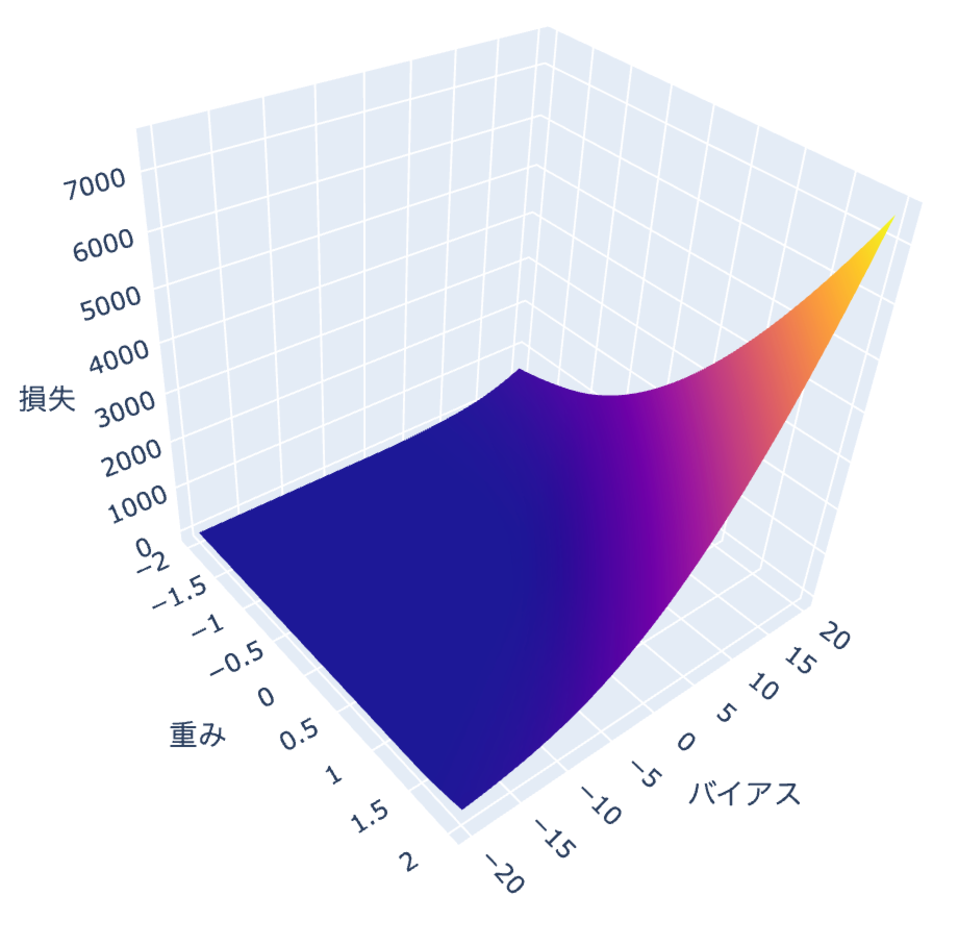
\includegraphics[width=0.7\linewidth]{fig/1-dim-relu-3d.pdf}

  \caption{三角関数を用いたToekn Encoding.}
\label{fig:tri-pos-encoding}

この処理をToekn Embeddingで用いた例に適応させる。
\end{figure}

\begin{equation*}
  \text{具体例}
\end{equation*}

この様にpositional encodingの適用後は、ベクトルが単語の意味だけでなく文章中の位置も含むようになり、その結果それぞれのベクトル(元々はトークン)を並列的に処理できるようになった。


\subsubsection{Attention}
attentionとは文中のの特定の箇所に注意を向けるように学習していく方法である。 この関数は入力として二つの変数 x と z を受け取り、 x=z の場合を特別にself attentionと呼ぶ。例えばxとして、翻訳元である日本語のトークン列、zとしては、翻訳先である英語のトークン列が対象となる。このattentionがtransformerの肝となる部品であるがその働きは直観的であり、人間が文章を読んだり翻訳する際に自然に行っている行為を再現した機構となっている。図~\ref{fig:att-abs}はattentionを直感的に説明する上で役立つ概念図である。(a)のself attentionはエンコーダ層・デコーダ層の両方に埋め込まれており、文章中の単語の意味を理解する際に、文章中のどの単語に注目するべきかを学習する。 (b)の通常のattentionはデコーダ層のみに埋め込まれており、翻訳先の文章中のある単語を生成するためには、翻訳元文章のどこに注目すれば良いかを学習する。


\begin{figure}
  \centering
    % 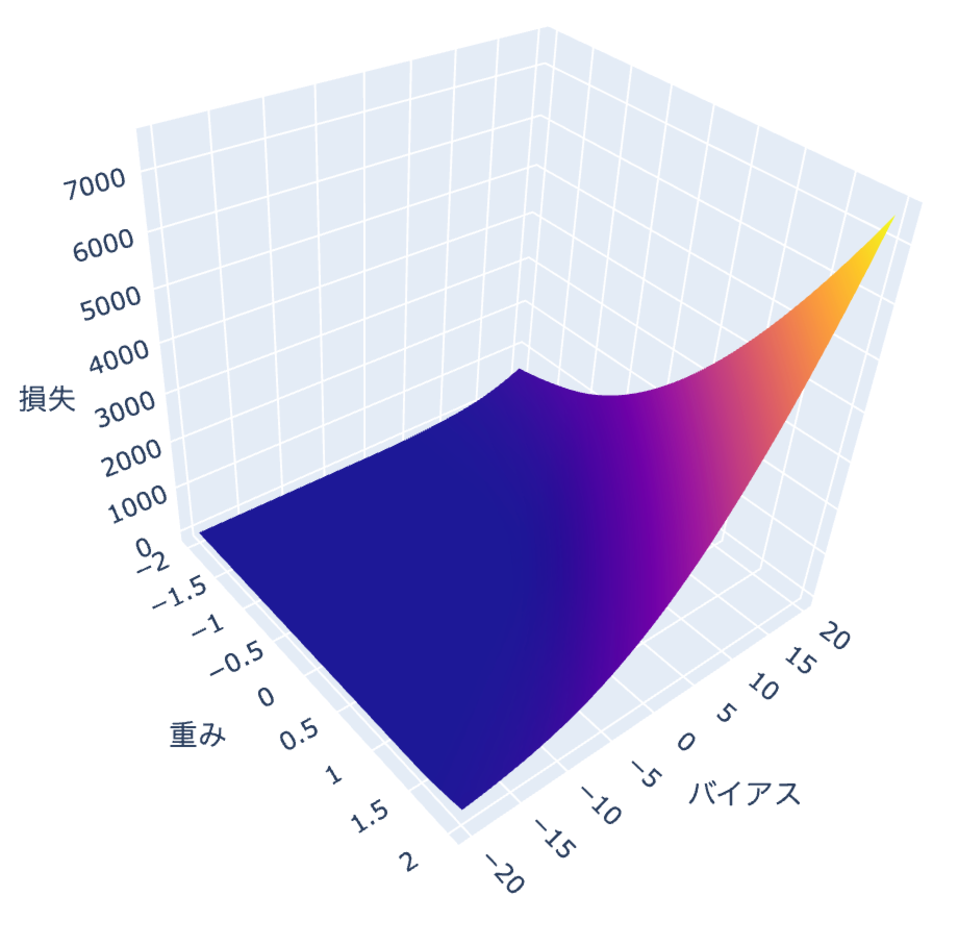
\includegraphics[width=0.7\linewidth]{fig/1-dim-relu-3d.pdf}

    (a) self attention
    \vspace{5mm}

    % 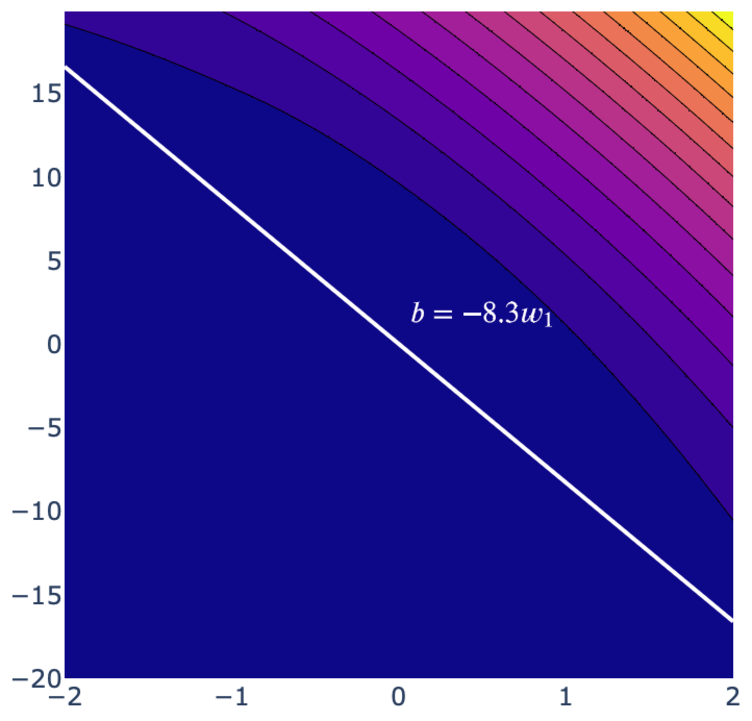
\includegraphics[width=0.7\linewidth]{fig/1-dim-relu-contour.pdf}
    (b) 通常のattention

  \caption{attentionの直観的な概念図}
\label{fig:att-abs}
\end{figure}

\subsubsection{Mask}

\begin{figure}
  \centering
  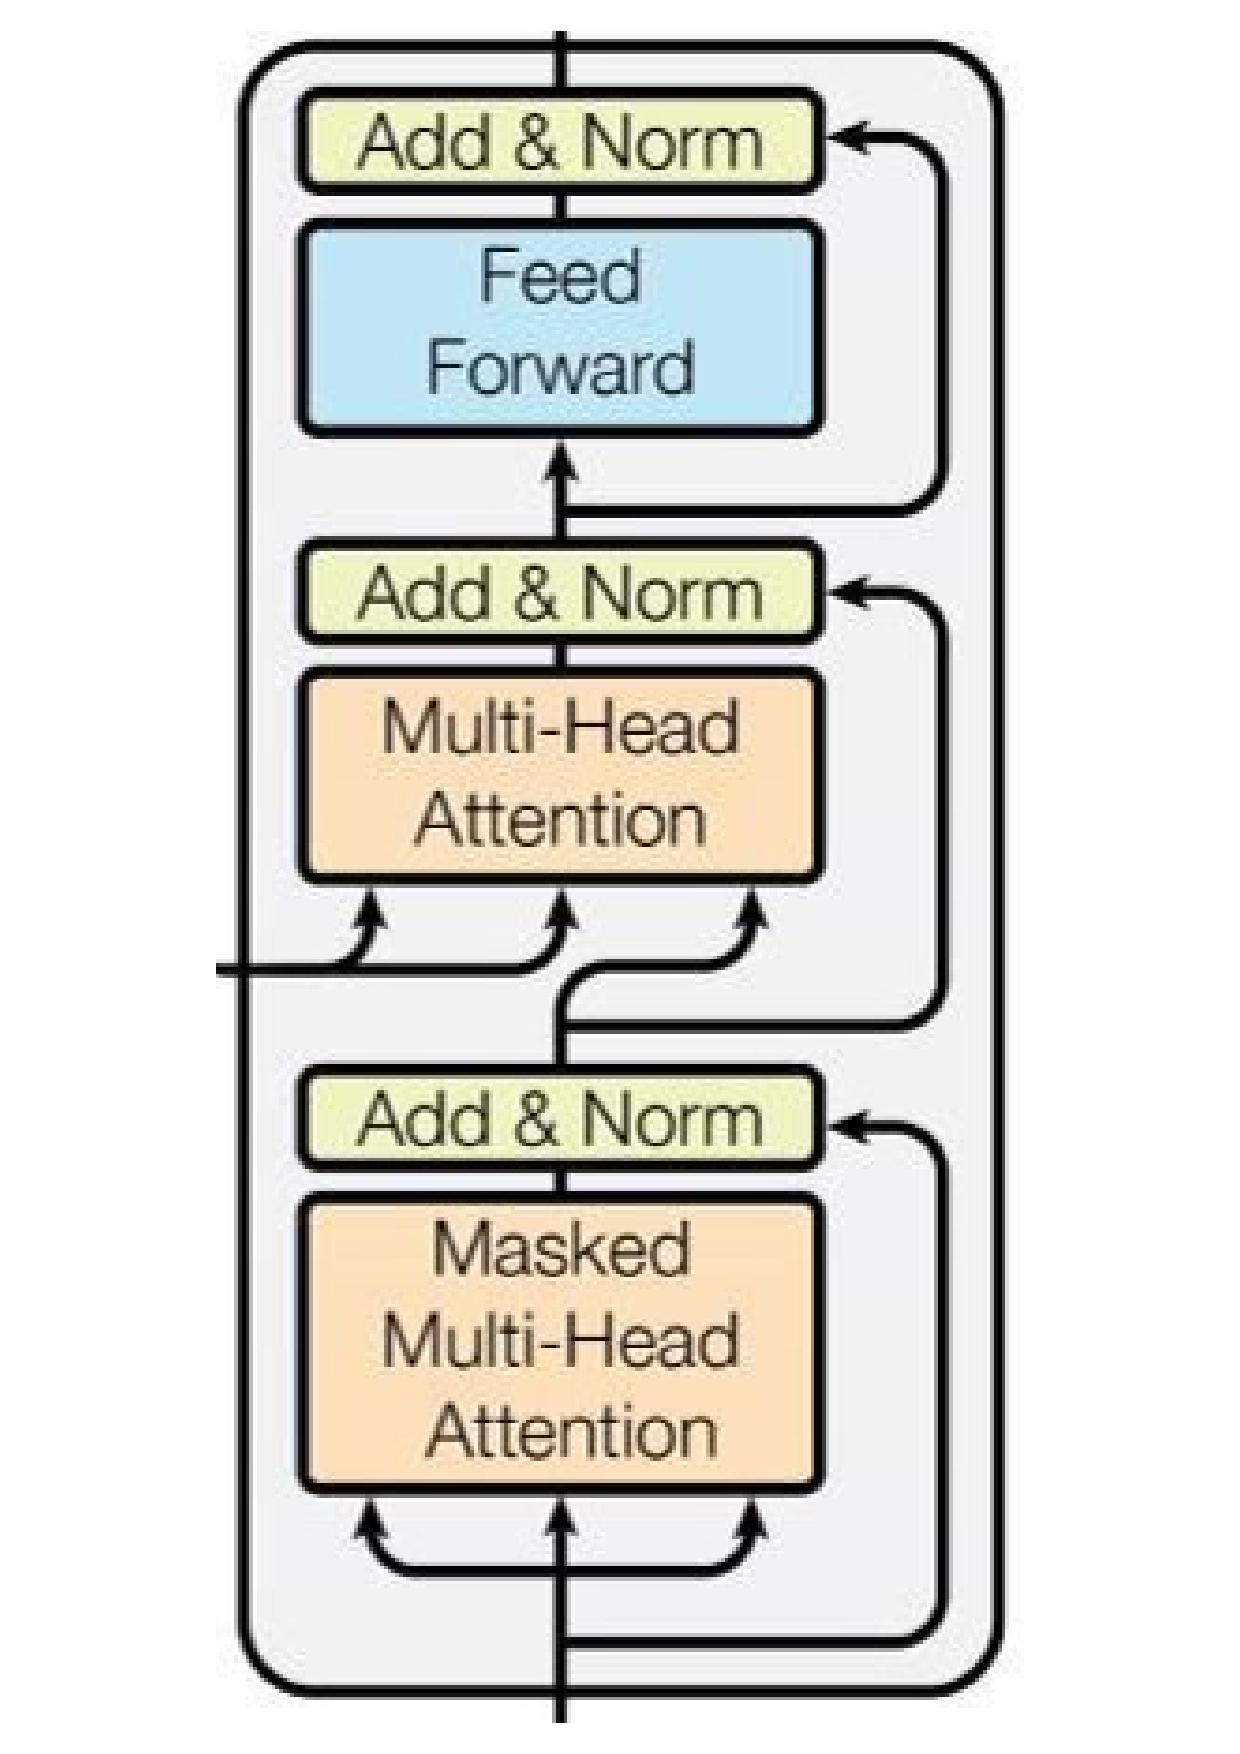
\includegraphics[width=0.5\linewidth]{fig/decoder.pdf}
  \caption{mask}
\label{fig:mask}
\end{figure}

Decoderにおけるself attentionには"Masked Attention"という特殊な名前が付いている。maskとは本来何かを覆い隠したりする意味である。transformerの場合は学習段階においてl番目のトークン$x_{l+1}$を予測する際に、それ以前のトークン情報のみを予測に使用するように、l+1以降のトークンを覆い隠す。言い換えると、mask機能を追加することでtransformerからの出力が式~(\ref{eq:trans})となることを保証する。

\subsubsection{学習}

まずは損失関数を定義する。文章対$(X, Z)$に対してtransformerからの出力$f_\theta(X_i, Z_i)$は
~(\ref{eq:trans})で表されるので、一つのデータ(文章対)に対する損失関数は交差エントロピーを用いて
\begin{equation}
  \label{eq:cross_trans}
  - \sum_{l=0}^{L-1} \log P_\theta(x_{l+1} | Z, x_0, \cdots, x_{l-1} )
\end{equation}
として定義される。
  \label{eq:cross_trans}
訓練データセットに$n$個の文章対$(X_1, Z_1),\ldots, (X_n, Z_n)$が含まれている場合は、損失関数は~(\ref{eq:cross_trans})の単純な足し合わせとして計算すればよい。この損失関数に対して勾配降下法などを用いて最適化をすることで、確率分布$P_\theta(x_{l+1} | Z, x_0, \cdots, x_{l-1} )$を理想の確率分布$P(x_{l+1} | Z, x_0, \cdots, x_{l-1} )$へと近づけていく。 

\subsubsection{推論}
実際に翻訳元の文章$Z = [z_0, z_1, .., z_{L^\prime}]$から翻訳先の文章$X = [x_0, x_1, .., x_{L}]$を生成する場合は、いわゆる\text{\bf{オンライン推論}}が用いられる。オンライン推論では$Z$から一度で翻訳先の文章$X$を生成するのではなく、左から順に一つづつ単語を生成していく。


\begin{equation*}
  \text{具体例}
\end{equation*}


\subsubsection{transformerを用いたモデル}